\documentclass[11pt]{article}
\usepackage[utf8]{inputenc}
\usepackage[spanish]{babel}
\usepackage{graphicx}
\usepackage{geometry} 
\usepackage{amsmath}
\usepackage{amssymb}
\usepackage[dvipsnames]{xcolor}
\usepackage{listings}
\usepackage{color}
\usepackage{float}
\usepackage{tcolorbox}
\usepackage{booktabs}

\lstset{
	language=R,
	basicstyle=\ttfamily,
} % listing definido para el lenguaje R

\geometry{letterpaper, 
	left= 3cm,
	right= 2.5cm,
	top= 2.5 cm,
	bottom= 2.5 cm} % Márgenes de la hoja

\newtcolorbox[auto counter, number within=section]{commentbox}[2][]{colback=beige!90!white, colframe=beige!50!black, fonttitle=\bfseries, title=Comentario~\thetcbcounter: #2, #1}
% Ajustes para tcolorbox


\begin{document}
	
	% Portada de la tarea
	\begin{titlepage}
		
		\centering
		
\includegraphics[width=0.2\textwidth]{logo_universidad} %logo de la universidad
		\hspace*{0.4\textwidth}
		
\includegraphics[width=0.2\textwidth]{images}\par\vspace{0.3cm} %logo de la facultad
		{\color{black}\rule{\textwidth}{4pt}}\\
		\vspace{1cm}
		{\bfseries\LARGE Nombre de la universidad}\\
		\vspace{1cm}
		{\scshape\Large Licenciatura}\\
		\vspace{1cm}
		{\color{black}\rule{\textwidth}{4pt}}\\
		\vspace{3cm}
		{\scshape\Huge Nombre de la materia}\\
		\vspace{3cm}
		{\itshape\Huge Tarea X}\\
		\vfill
		{\Large Alumno: }\\
		{\Large Nombre del alumno}\\
		\vfill
		{\Large \today}\\ % fecha por defecto
		
	\end{titlepage}
	% Comenzamos enumerando los probelas con enumerate
	\begin{enumerate}
		% ejemplo de un ejercicio
		\item Gráfica en R los siguientes datos y realiza una regresión lineal en R:
		$$ x = \{1,2,3,4,5,6,7,8,9,10,11,12,13,14,15\}$$
		$$ y = \{2, 5, 7, 11, 16, 17, 19, 20, 25, 30, 29, 31, 40, 42, 45 \}$$ 
		
		\textbf{Solución.}
		% bloque para el código R
		\begin{lstlisting}
x <- c(1,2,3,4,5,6,7,8,9,10,11,12,13,14,15)
y <- c(2,5,7,11,16,17,19,20,25,30,29,31,40,42,45)
plot(x, y, main = "Grafica de dispersion")

lm.modelo <- lm(y ~ x)
summary(lm.modelo)

Call:
lm(formula = y ~ x)

Residuals:
Min      1Q  Median      3Q     Max 
-3.5857 -0.6107  0.3786  1.4143  2.4179 

Coefficients:
Estimate Std. Error t value Pr(>|t|)    
(Intercept)  -1.3714     1.0176  -1.348    0.201    
x             2.9964     0.1119  26.773 9.33e-13 ***
---

Residual standard error: 1.873 on 13 degrees of freedom
Multiple R-squared:  0.9822,	Adjusted R-squared:  0.9808 
F-statistic: 716.8 on 1 and 13 DF,  p-value: 9.331e-13
		\end{lstlisting}
	
	% insersión de imagenes
		\begin{figure}[h!]
		\centering
		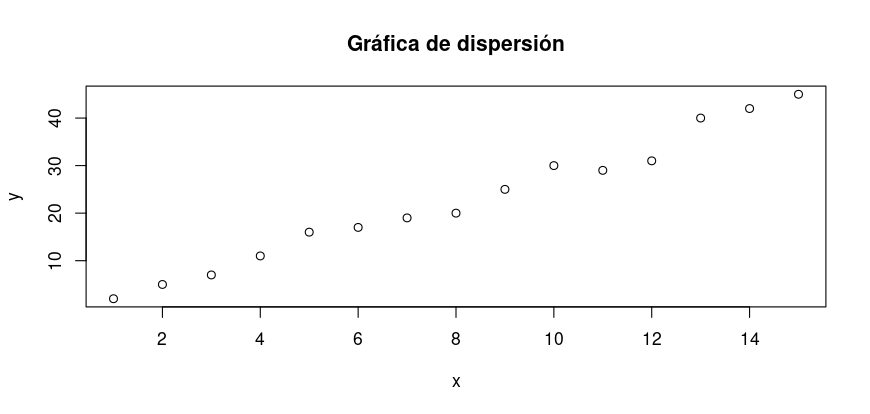
\includegraphics[width=1\textwidth]{image1}
		\end{figure}
	
		\item Calcule lo siguiente: 
		\begin{itemize}
			\item[i)] Media de $x$:
		% uso de tcolorbox
		\begin{tcolorbox}
		$$\bar{x} = \frac{\sum_{i=1}^{n}}{n} = 8$$
		\end{tcolorbox}
			\item[ii)] Media de $y$:
		\begin{tcolorbox}
			$$\bar{x} = \frac{\sum_{i=1}^{n}}{n} = 22.6$$
		\end{tcolorbox}
		\end{itemize}
		
	\end{enumerate}
\end{document}
